\documentclass[10pt]{beamer}
\usepackage{hyperref}
\usepackage{bm}
\usepackage[
    style=authoryear,
    backend=biber
]{biblatex}
\usepackage{caption}
\captionsetup[figure]{labelformat=empty, font=scriptsize}

\usetheme{wur}

\title{Programming for the web}
\subtitle{An introduction to front-end development with React}
\author{Rens Holmer}
\institute{Wageningen University -- Bioinformatics}

\setbeamertemplate{navigation symbols}{}

\begin{document}

\begin{frame}
    \titlepage
    \begin{figure}
        
\includegraphics[width=.7\linewidth]{figures/get-in-loser.pdf}
    \end{figure}
\end{frame}

\begin{frame}{Web development in bioinformatics}
    \begin{figure}
        \begin{minipage}{.3\linewidth}
            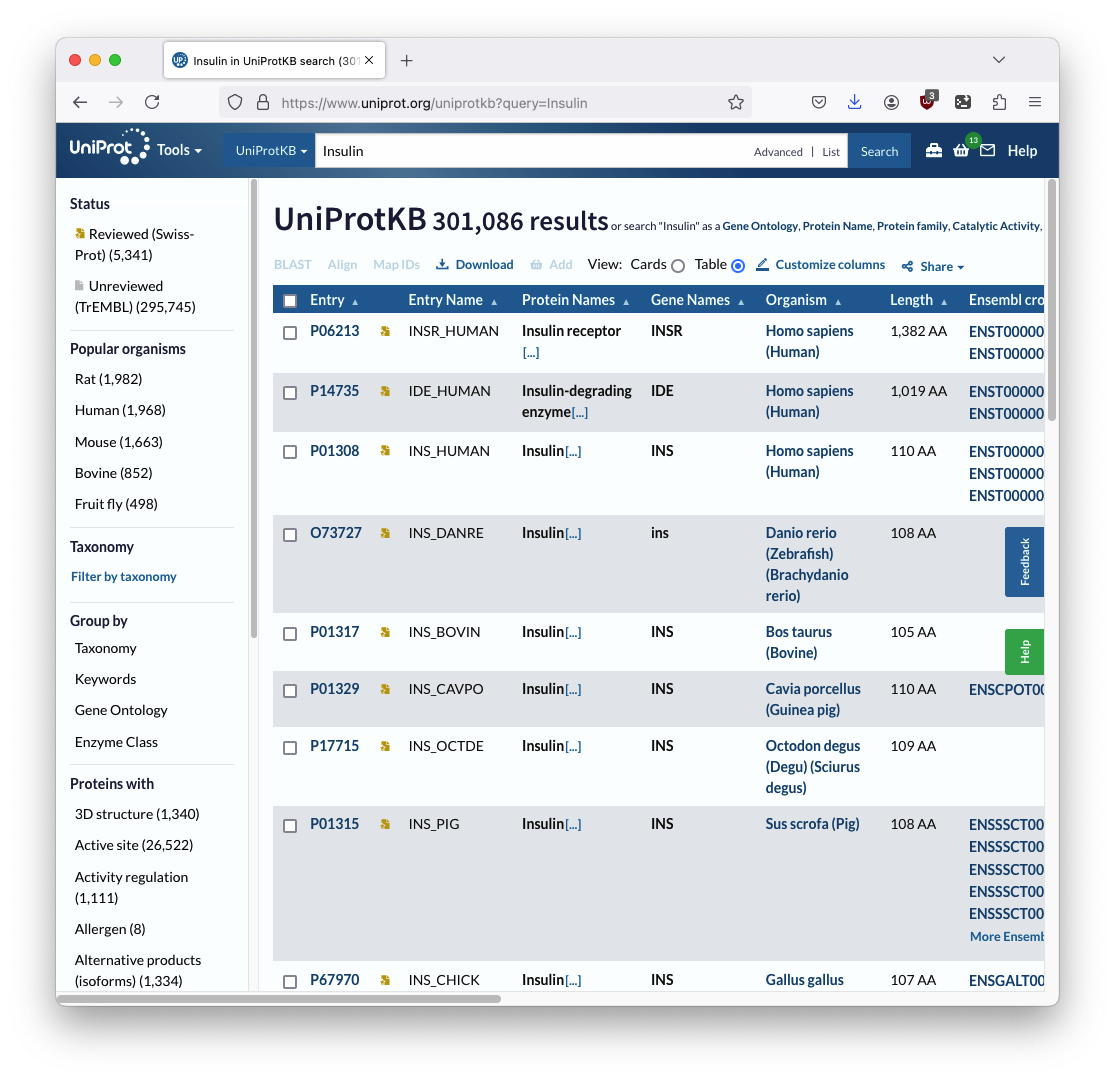
\includegraphics[
                width=\linewidth
            ]{figures/uniprot.png}
            \\ \tiny{Uniprot}
        \end{minipage}
        \begin{minipage}{.3\linewidth}
            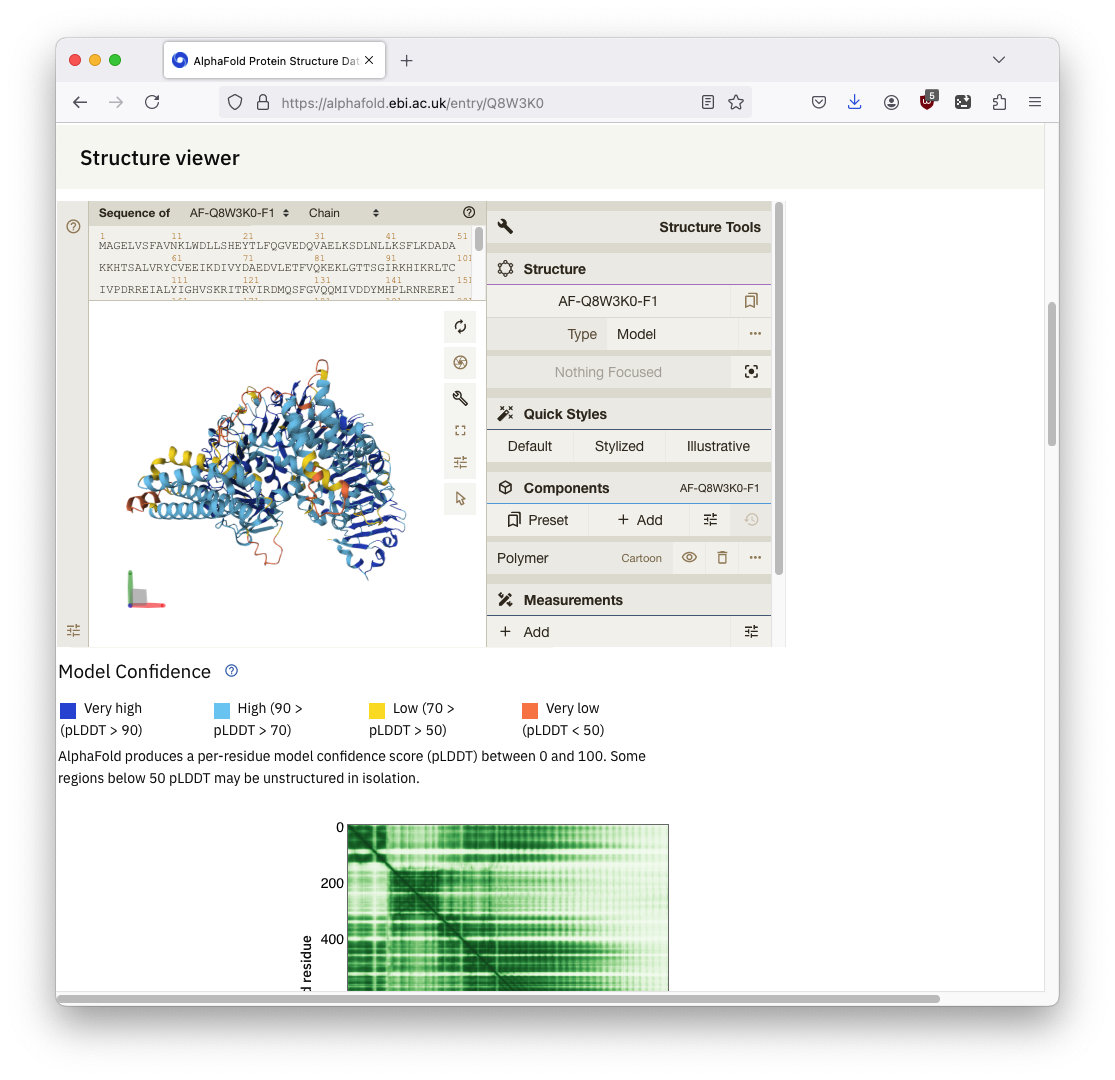
\includegraphics[
                width=\linewidth
            ]{figures/alphafold-db.png}
            \\ \tiny{Alphafold-DB}
        \end{minipage}
    \end{figure}
    \begin{figure}
        \begin{minipage}{.3\linewidth}
            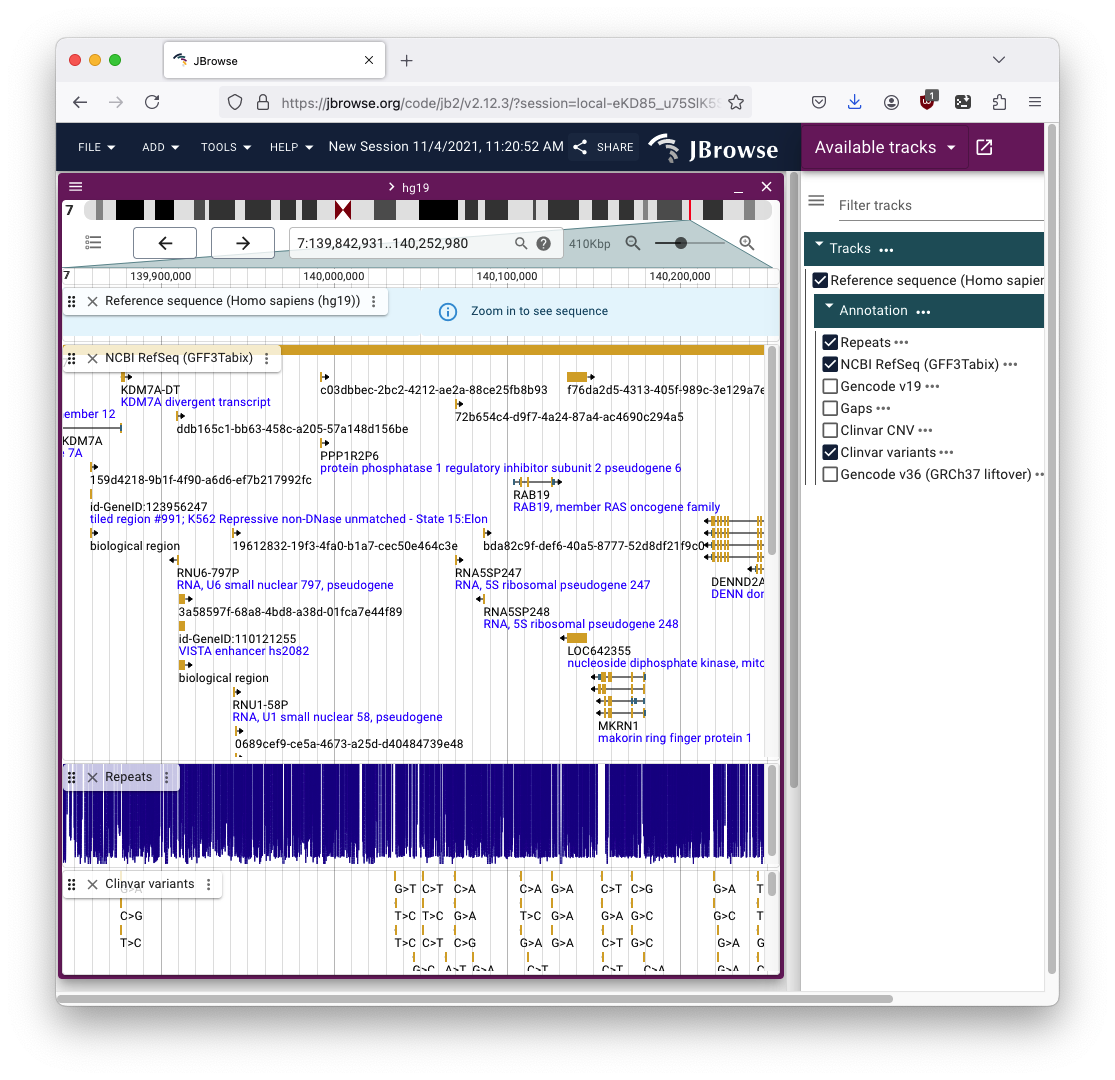
\includegraphics[
                width=\linewidth,
            ]{figures/jbrowse.png}
            \\ \tiny{JBrowse}
        \end{minipage}
        \begin{minipage}{.3\linewidth}
            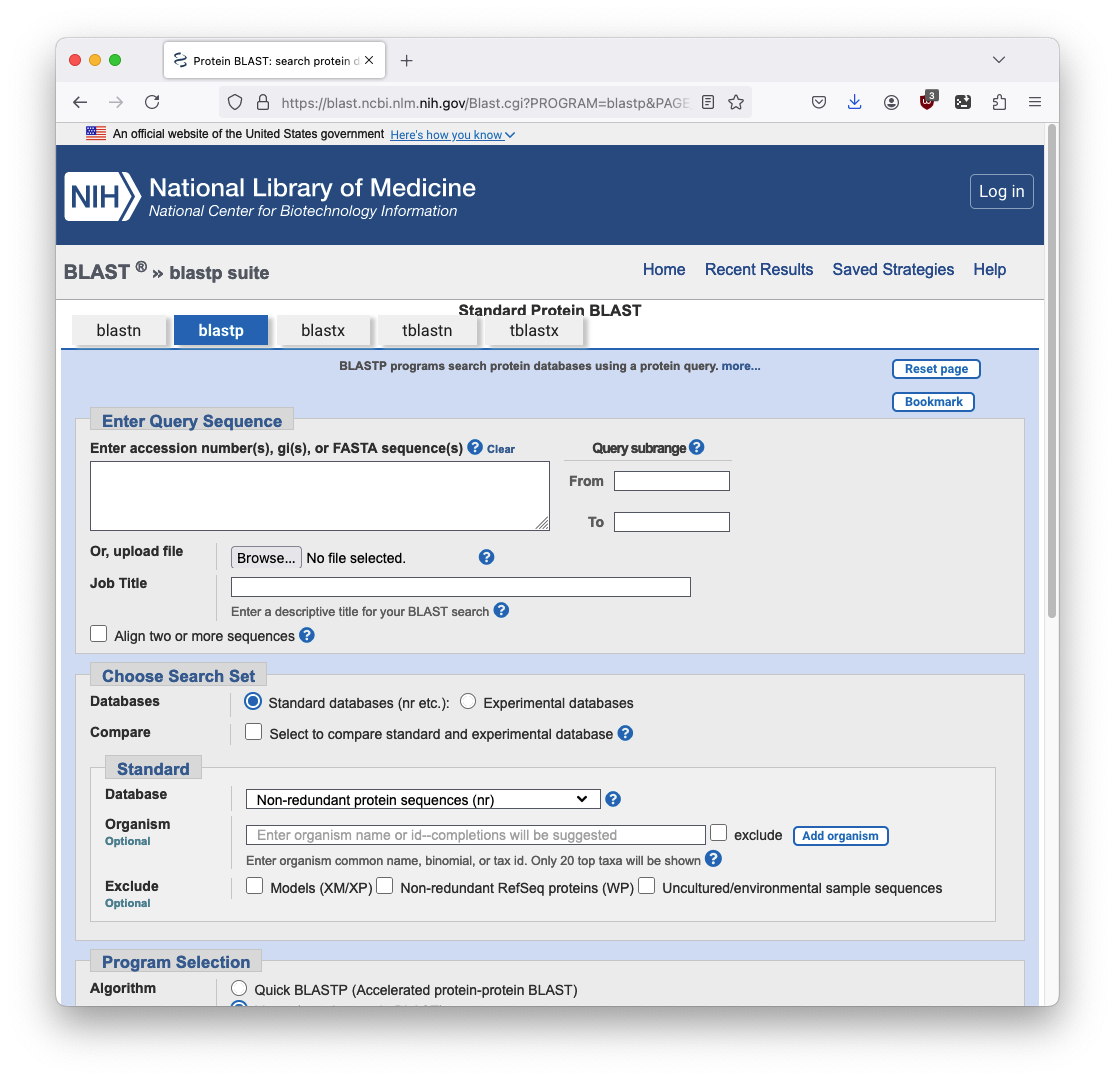
\includegraphics[
                width=\linewidth,
            ]{figures/ncbi-blast.png}
            \\ \tiny{NCBI BLAST}
        \end{minipage}
    \end{figure}
\end{frame}

\begin{frame}

    {\huge Goal of this session}
    \begin{itemize}
        \item Introduction to building \textit{interactive} websites
    \end{itemize}
    \vspace{2em}
    {\large Activities}
    \begin{itemize}
        \item Familiarize yourself with main building blocks of a website
        \item Learn about modern toolchains and frameworks for the web
        \item Build your own interactive bioinformatics data visualization
    \end{itemize}
    \vspace{1em}
    {\large Material}
    \begin{figure}
        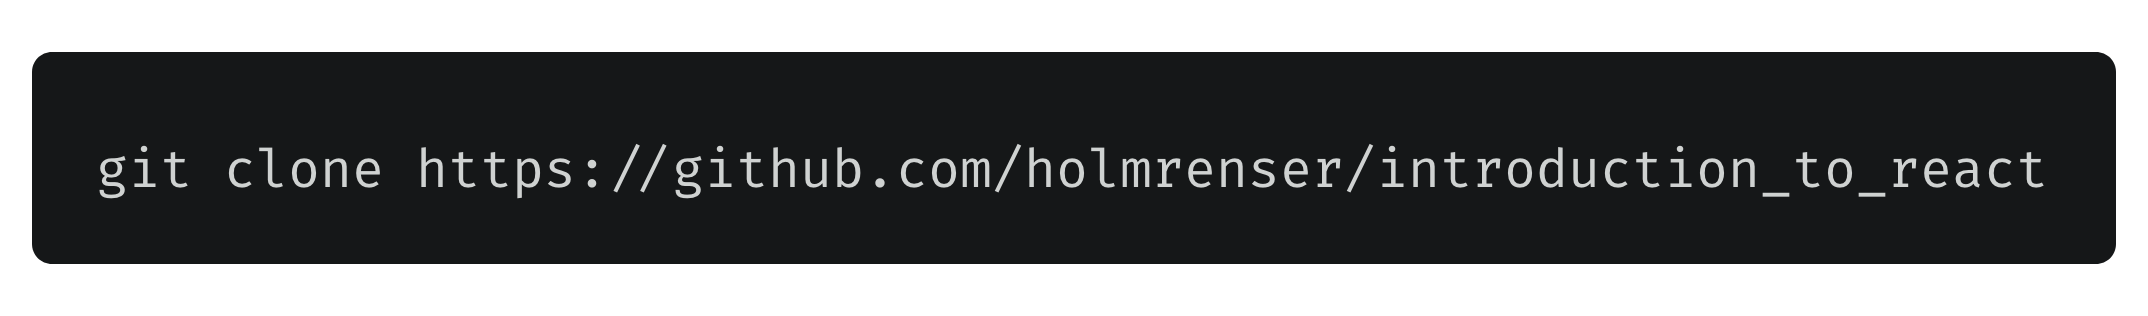
\includegraphics[width=.99\linewidth]{figures/material-link.png}
    \end{figure}
\end{frame}

\begin{frame}

    {\huge Assignment 1}

    \vspace{1em}
    Explore two versions of a simple static website:

    \vspace{.5em}

    \texttt{example/simple\_site}

    \texttt{example/simple\_site\_single\_file}


    \vspace{2em}
    \begin{itemize}
        \item Open the workshop folder in an IDE (e.g. VSCode)
        \item Open \texttt{index.html} in a web browser
        \item Open the developer tools (\texttt{cmd + shift + C})
        \item Click the button
        \item Explore the code
        \item \textit{Discuss}
    \end{itemize}
\end{frame}

\begin{frame}{Some technical background}

    {\LARGE Core components}

    \begin{itemize}
        \item {\large HTML:} HyperText Markup Language, i.e. text with links and sematics for 'function' such as headers or links.
        \item {\large JS:} JavaScript, actions, interaction, Document Object Model (DOM).
        \item {\large CSS:} Cascading Style Sheets, visual styling. Style applies to HTML tag and all it's children (hence 'cascading').
    \end{itemize}
    \vspace{2em}

    {\LARGE Key concepts}

    \begin{itemize}
        \item \underline{Asynchronous programming:} networks can be slow, local computation should not wait (examples in next slides)
        \item Using the browser as a debugger and REPL
    \end{itemize}
\end{frame}

\begin{frame}

    {\huge We have to talk about AJAX}

    \begin{itemize}
        \item \underline{A}synchronous \underline{J}avascript \underline{A}nd \underline{X}ml
        \item Originally introduced as concept for typical web tasks
        \item Does not actually have to use XML (today we use JSON)
        \item Modern JS: implemented in e.g. \texttt{fetch} API
    \end{itemize}

    \begin{figure}
        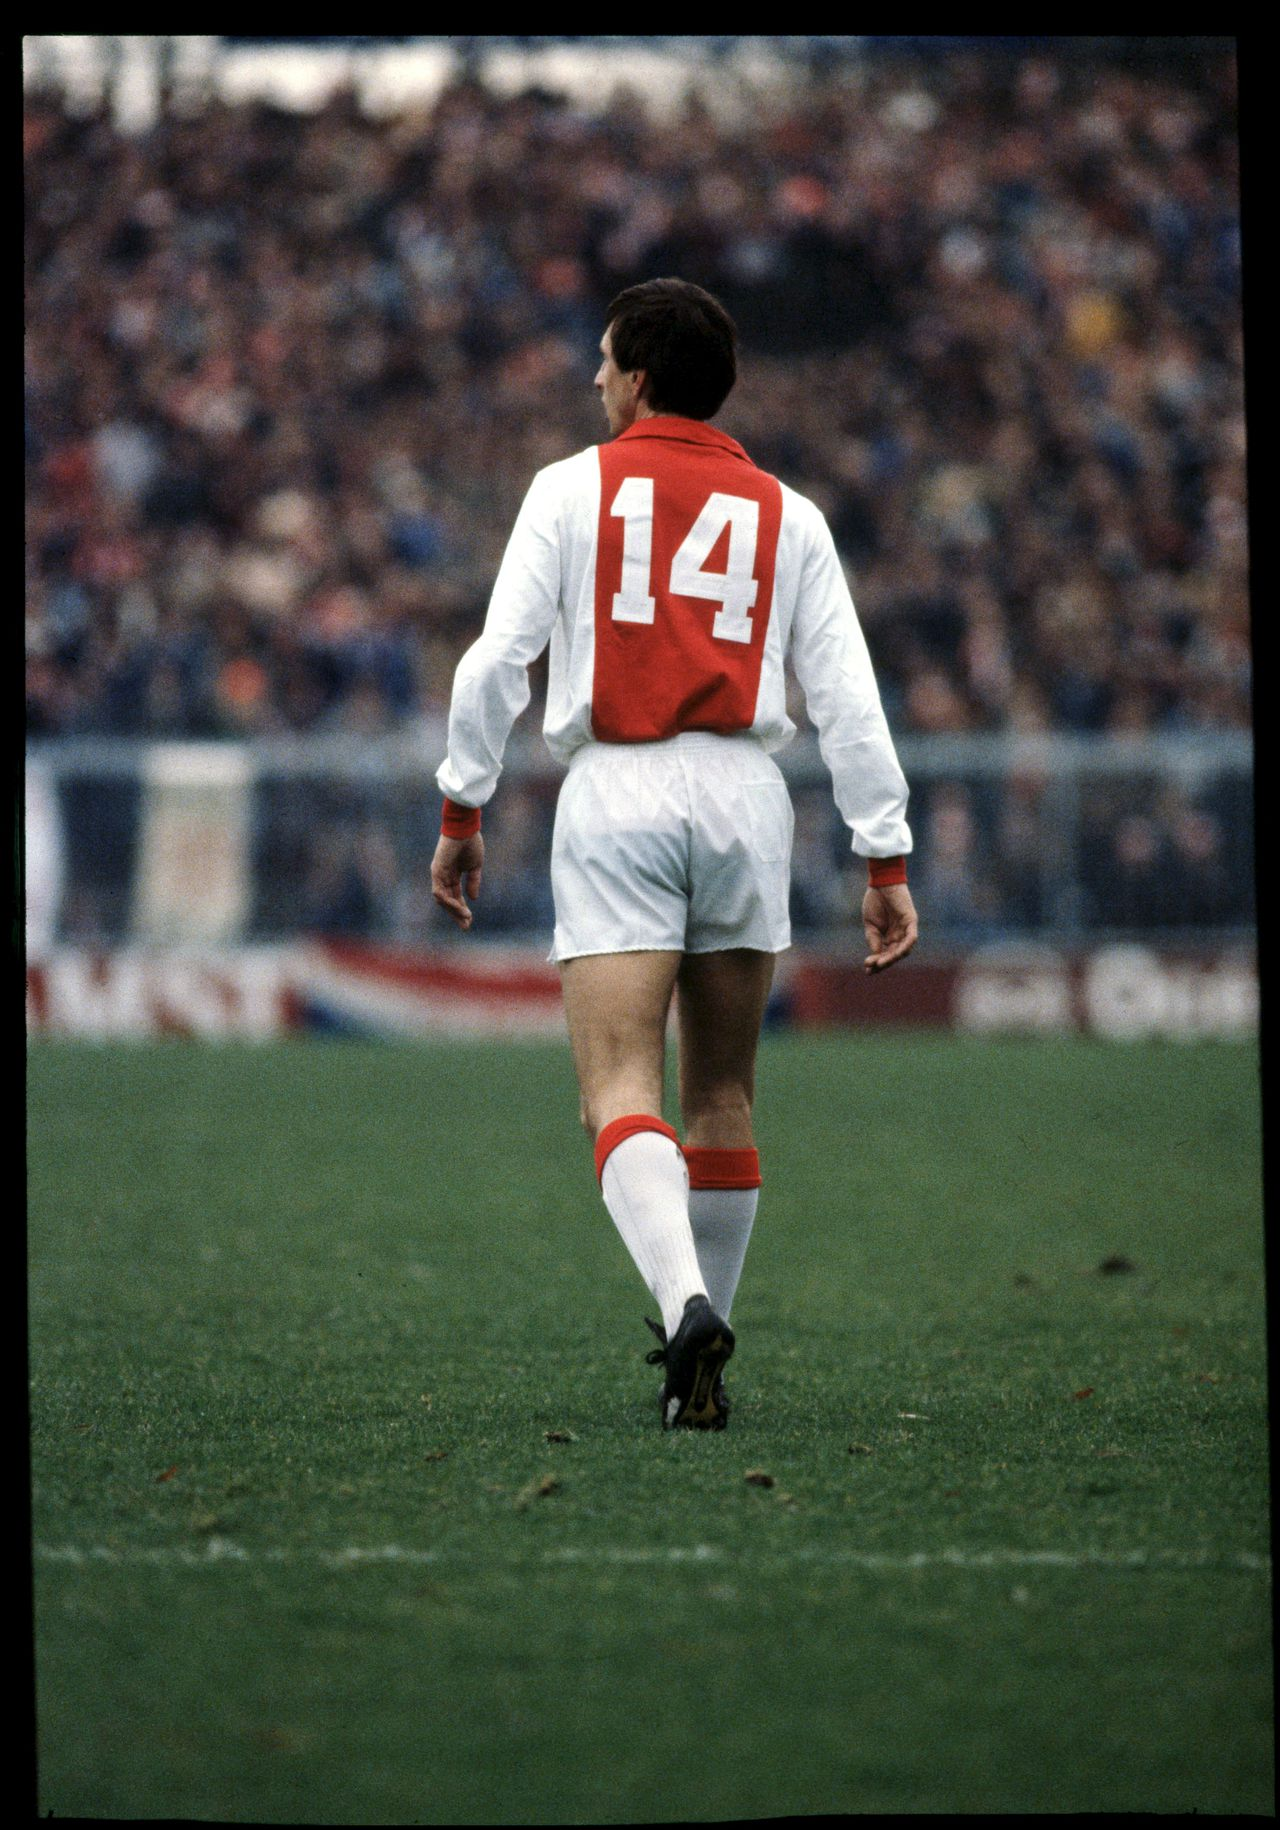
\includegraphics[
            width=.25\linewidth,
            trim={4cm 10cm 4cm 4cm},
            clip
        ]{figures/cruijf.jpg}
        \\
        {\tiny The other AJAX}
    \end{figure}
\end{frame}

\begin{frame}{Event loop}
    On the web, we send requests and respond \textit{asynchronously}
    \begin{figure}
        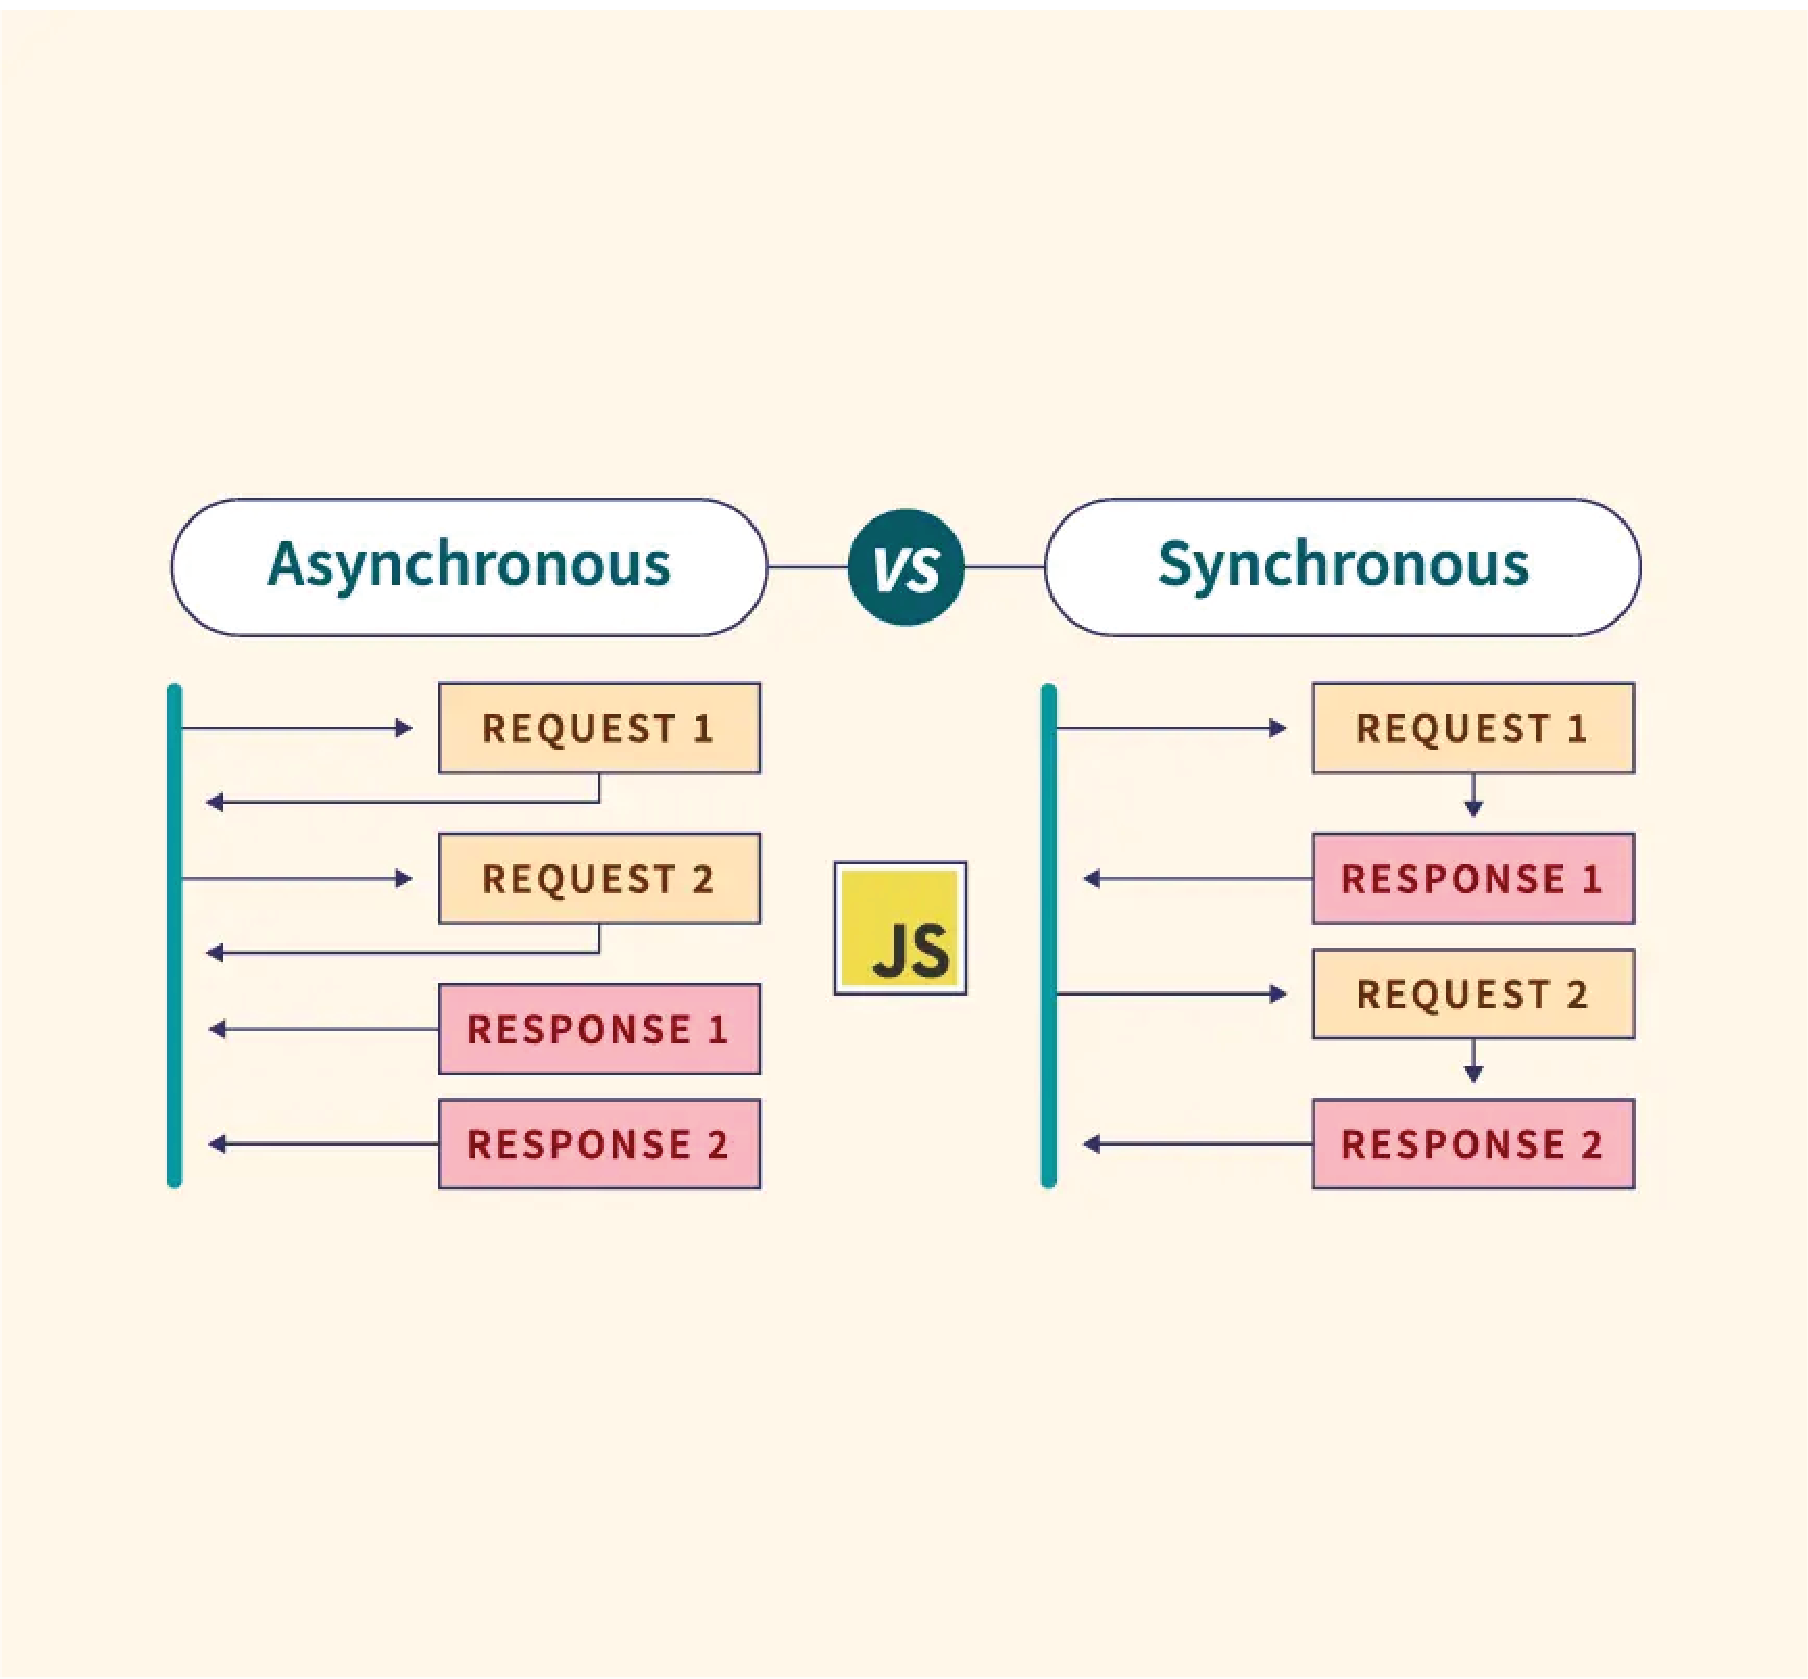
\includegraphics[
            width=.5\linewidth,
        ]{figures/event-loop.pdf}
    \end{figure}

\end{frame}

\begin{frame}{Javascript quirks {\small (variables)}}
    Many aspects of JS are superficially similar to Python
    \begin{figure}
        \begin{minipage}{.4\linewidth}
            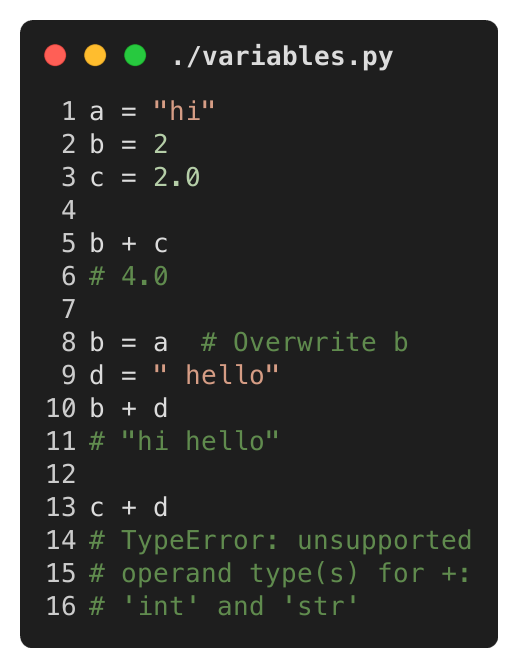
\includegraphics[
                width=\linewidth,
            ]{figures/variables.py.png}
            \\ \tiny{Python}
        \end{minipage}
        \begin{minipage}{.35\linewidth}
            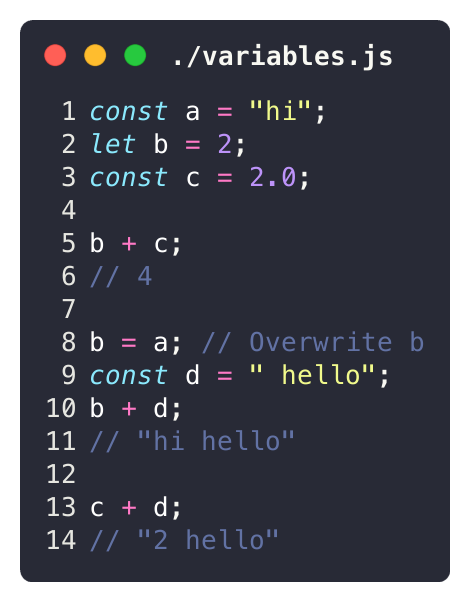
\includegraphics[
                width=\linewidth,
            ]{figures/variables.js.png}
            \\ \tiny{Javascript}
        \end{minipage}
    \end{figure}
\end{frame}

\begin{frame}{Javascript quirks {\small (functions)}}
    \begin{figure}
        \begin{minipage}{.45\linewidth}
            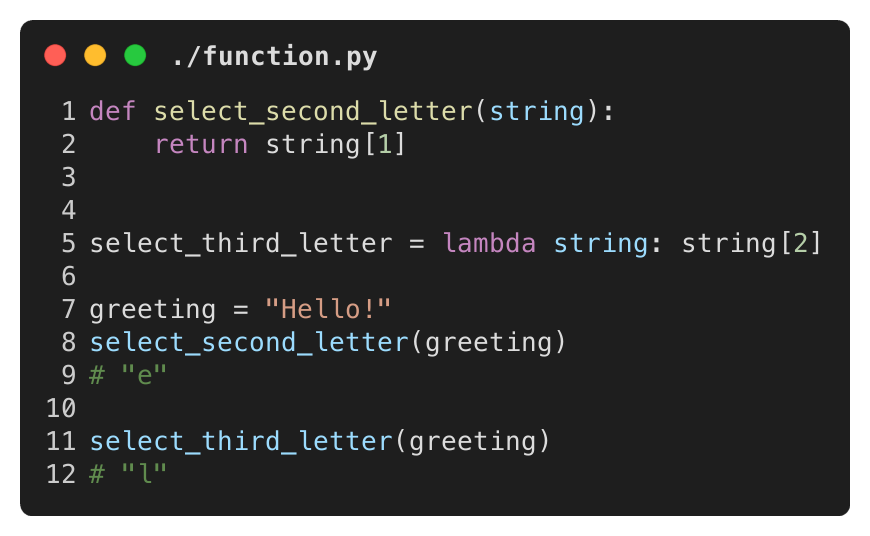
\includegraphics[
                width=\linewidth,
            ]{figures/function.py.png}
            \\ \tiny{Python}
        \end{minipage}
        \begin{minipage}{.45\linewidth}
            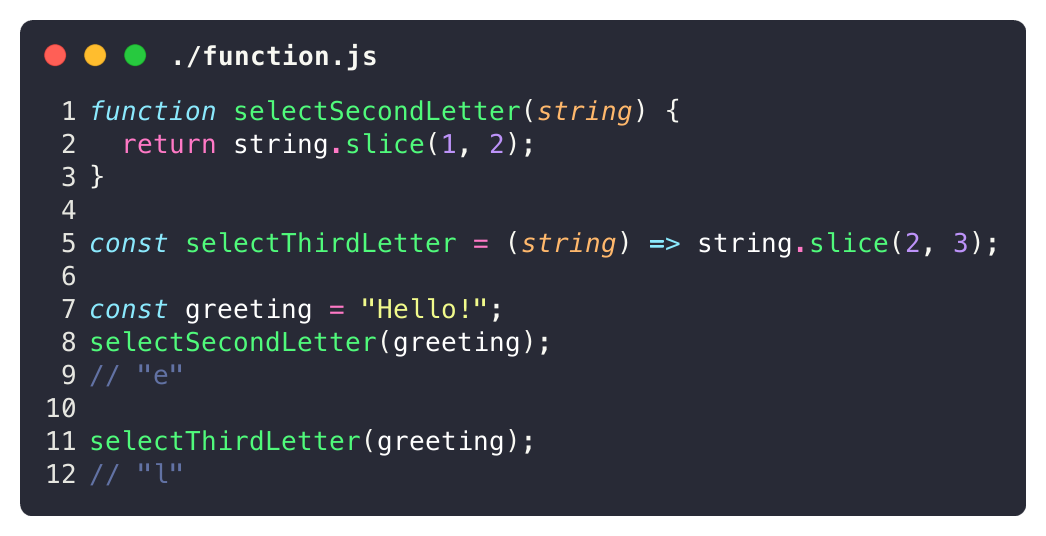
\includegraphics[
                width=\linewidth,
            ]{figures/function.js.png}
            \\ \tiny{Javascript}
        \end{minipage}
    \end{figure}
\end{frame}

\begin{frame}{Javascript quirks {\small (classes)}}
    \begin{figure}
        \begin{minipage}{.45\linewidth}
            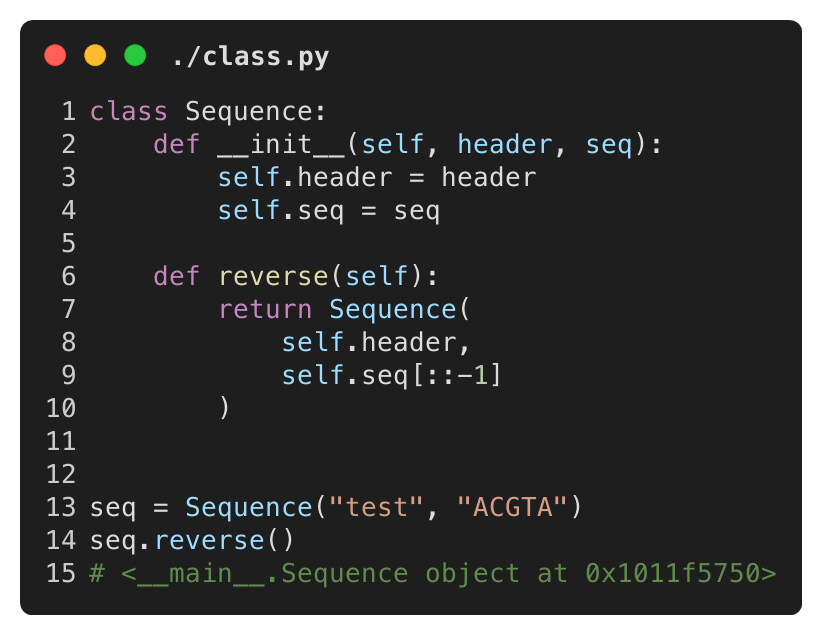
\includegraphics[
                width=\linewidth,
            ]{figures/class.py.png}
            \\ \tiny{Python}
        \end{minipage}
        \begin{minipage}{.45\linewidth}
            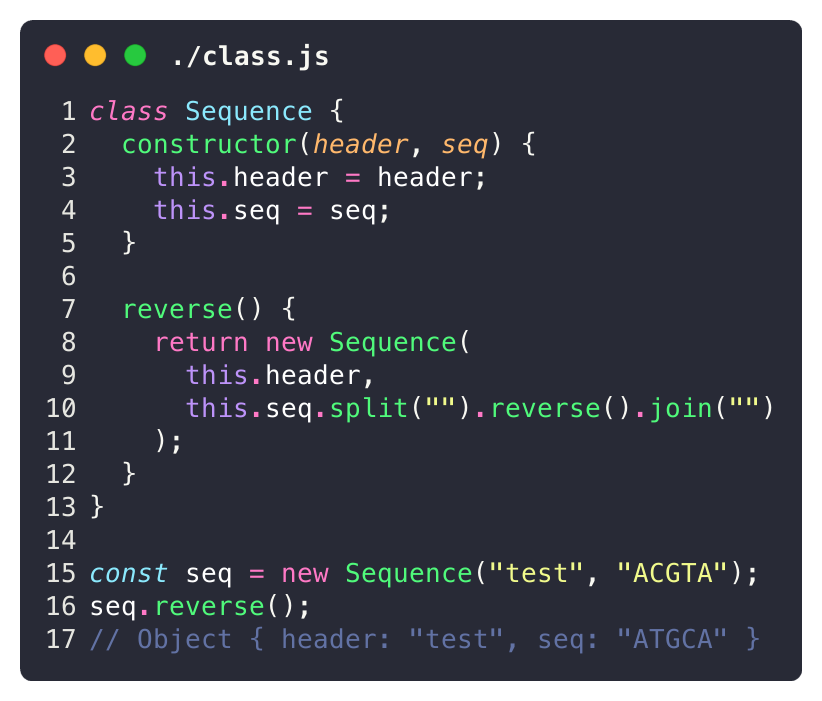
\includegraphics[
                width=\linewidth,
            ]{figures/class.js.png}
            \\ \tiny{Javascript}
        \end{minipage}
    \end{figure}
\end{frame}

\begin{frame}{Javascript quirks {\small (operations)}}
    \begin{figure}
        \begin{minipage}{.4\linewidth}
            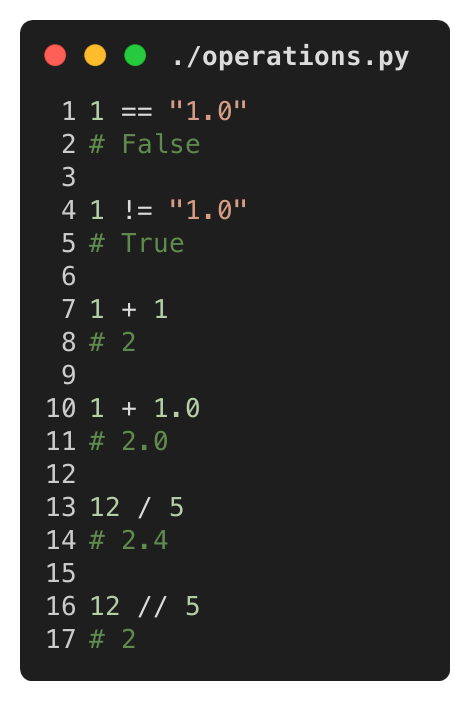
\includegraphics[
                width=\linewidth,
            ]{figures/operations.py.png}
            \\ \tiny{Python}
        \end{minipage}
        \begin{minipage}{.4\linewidth}
            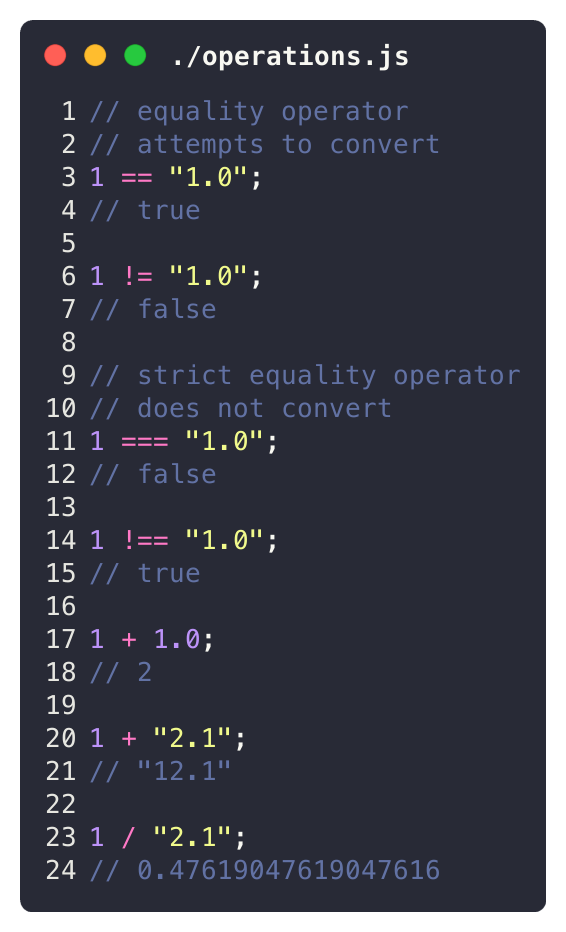
\includegraphics[
                width=\linewidth,
            ]{figures/operations.js.png}
            \\ \tiny{Javascript}
        \end{minipage}
    \end{figure}
\end{frame}

\begin{frame}{Javascript quirks {\small (types)}}
    \begin{figure}
        \begin{minipage}{.45\linewidth}
            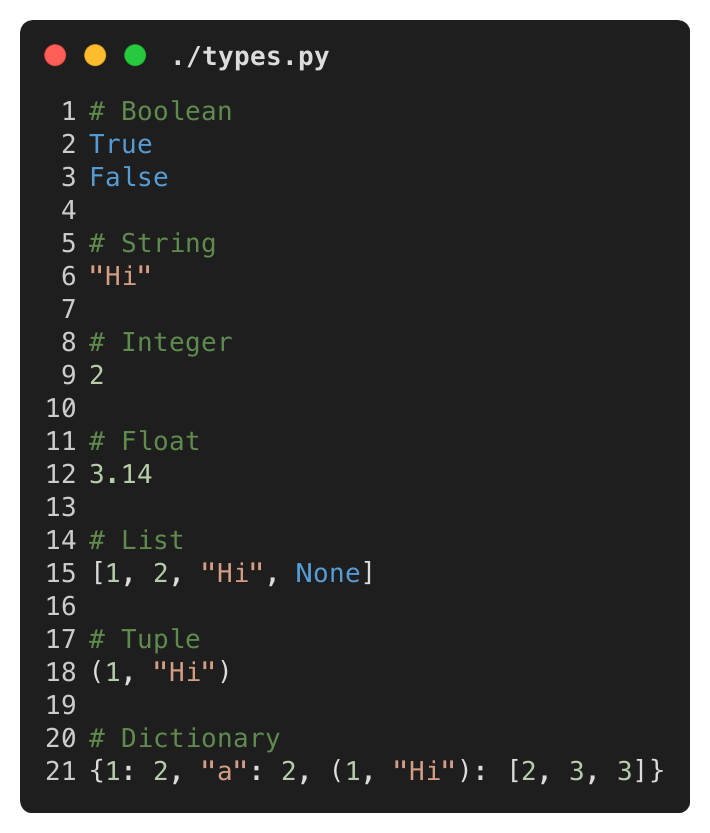
\includegraphics[
                width=\linewidth,
            ]{figures/types.py.png}
            \\ \tiny{Python}
        \end{minipage}
        \begin{minipage}{.45\linewidth}
            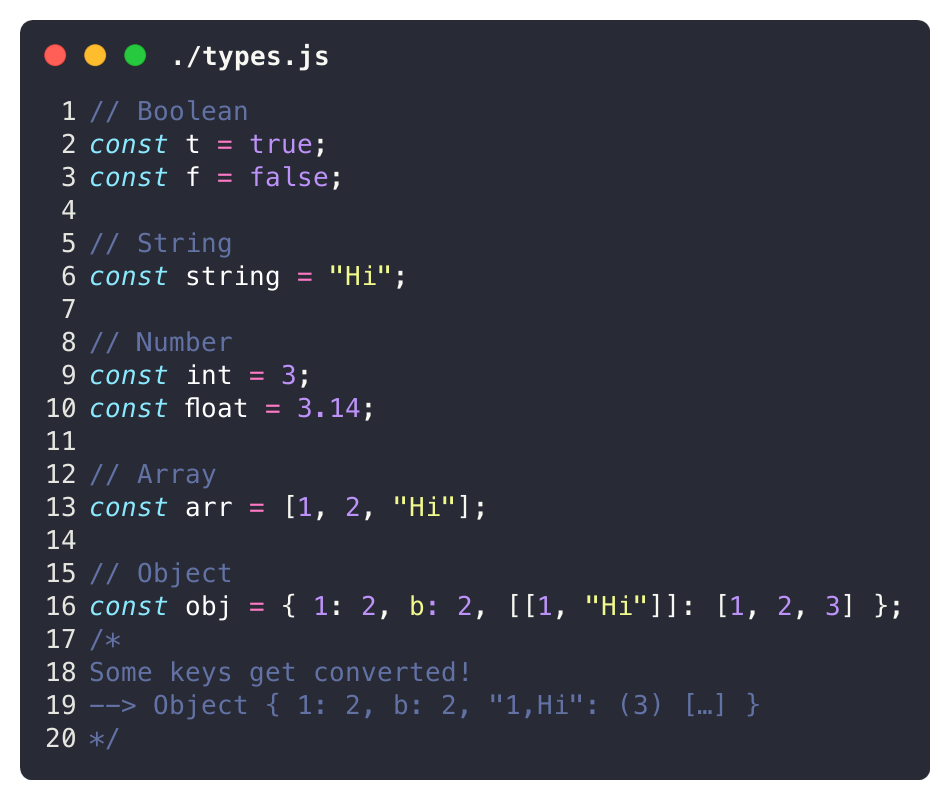
\includegraphics[
                width=\linewidth,
            ]{figures/types.js.png}
            \\ \tiny{Javascript}
        \end{minipage}
    \end{figure}
\end{frame}

\begin{frame}{Javascript quirks {\small (comments)}}
    \begin{figure}
        \begin{minipage}{.45\linewidth}
            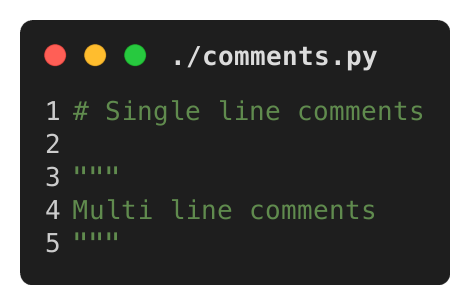
\includegraphics[
                width=\linewidth,
            ]{figures/comments.py.png}
            \\ \tiny{Python}
        \end{minipage}
        \begin{minipage}{.45\linewidth}
            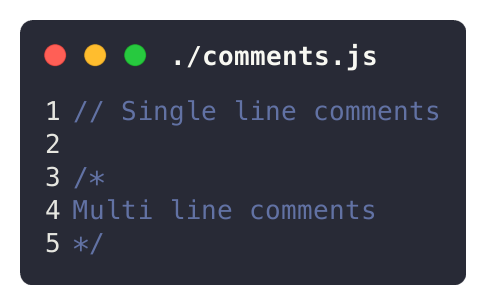
\includegraphics[
                width=\linewidth,
            ]{figures/comments.js.png}
            \\ \tiny{Javascript}
        \end{minipage}
    \end{figure}
\end{frame}

\begin{frame}{Javascript quirks {\small (controlflow)}}
    \begin{figure}
        \begin{minipage}{.45\linewidth}
            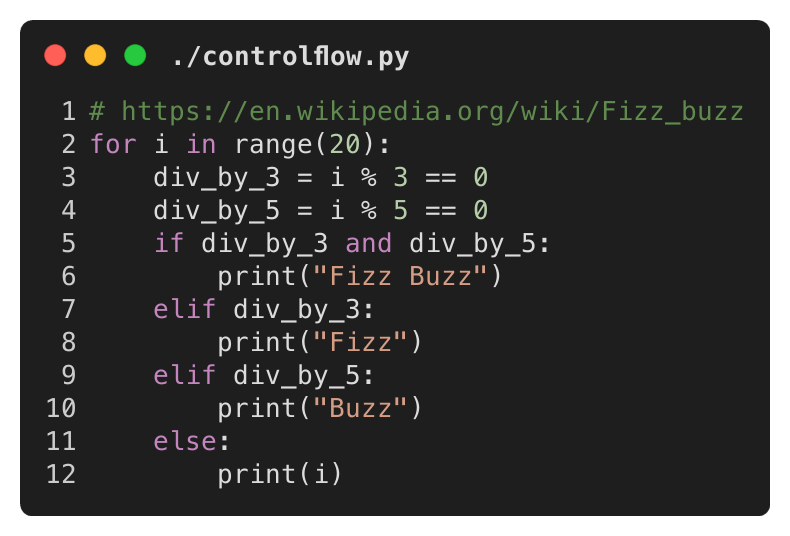
\includegraphics[
                width=\linewidth,
            ]{figures/controlflow.py.png}
            \\ \tiny{Python}
        \end{minipage}
        \begin{minipage}{.45\linewidth}
            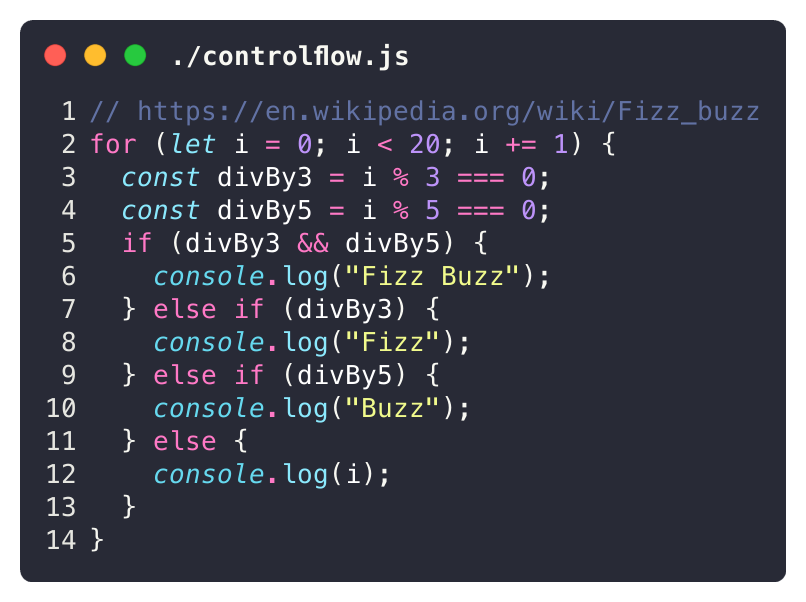
\includegraphics[
                width=\linewidth,
            ]{figures/controlflow.js.png}
            \\ \tiny{Javascript}
        \end{minipage}
    \end{figure}
\end{frame}

\begin{frame}{Javascript quirks {\small (string formatting)}}
    \begin{figure}
        \begin{minipage}{.45\linewidth}
            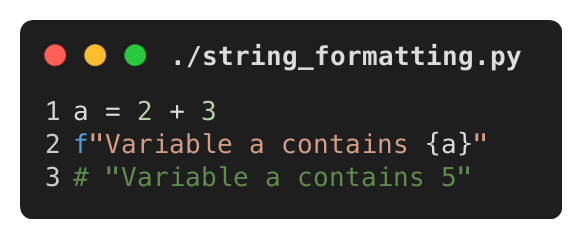
\includegraphics[
                width=\linewidth,
            ]{figures/string_formatting.py.png}
            \\ \tiny{Python}
        \end{minipage}
        \begin{minipage}{.45\linewidth}
            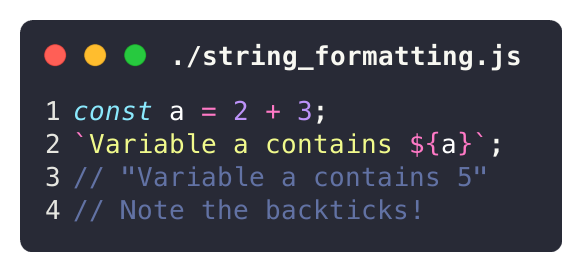
\includegraphics[
                width=\linewidth,
            ]{figures/string_formatting.js.png}
            \\ \tiny{Javascript}
        \end{minipage}
    \end{figure}
\end{frame}

\begin{frame}{Modern JS}
    Increasingly large/complex designs result in modern framework approach: introduce template language that emphasizes modularity, 'transpile' to HTML, JS, CSS.

    \begin{itemize}
        \item Some common frameworks: \underline{React}, Vue, Angular, Svelte, etc.
        \item Transpiling/bundling
        \item Component re-use
        \item State management
    \end{itemize}
\end{frame}

\begin{frame}{Assigment 2}
    Build a React app for visualizing MSAs

    \begin{itemize}
        \item Explore created folder structure: \texttt{package.json}, \texttt{node\_modules}, \texttt{vite.config.js}, \texttt{eslintrc.cjs}, \texttt{index.html}
    \end{itemize}

    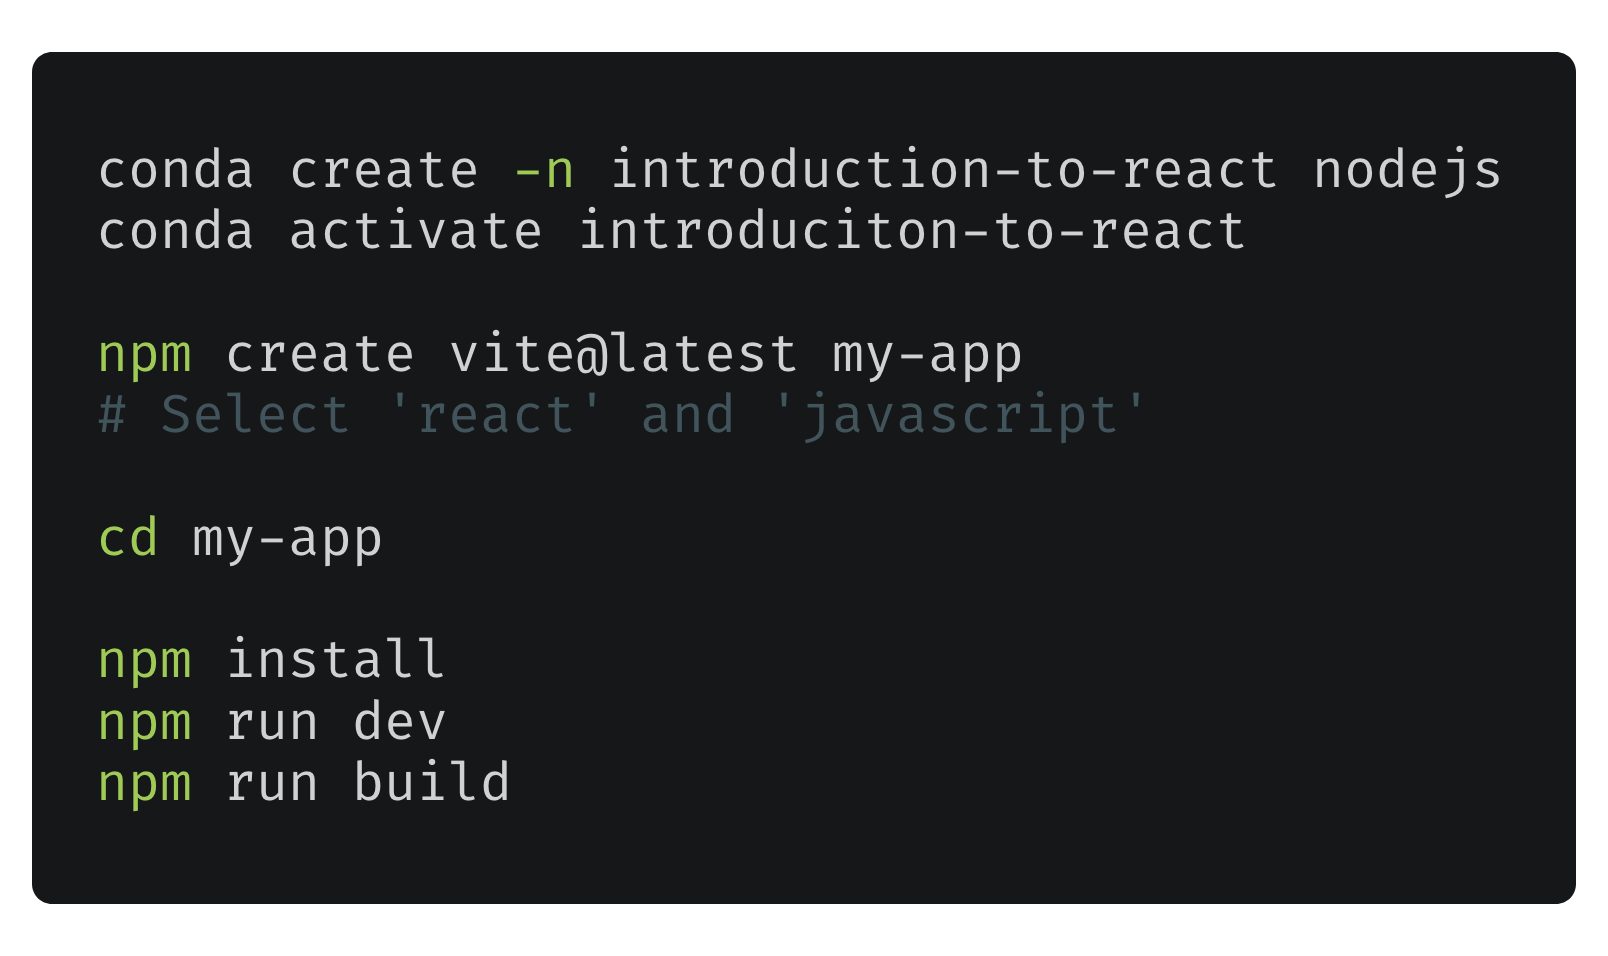
\includegraphics[
        width=.8\linewidth,
    ]{figures/initialize-app.png}
\end{frame}

\begin{frame}{Assignment 2 {\small continued}}
    Fetch some JSON data (available in the github repository of this tutorial)

    Example URL:

    \url{https://raw.githubusercontent.com/holmrenser/introduction_to_react/main/data/1.json}

    \begin{figure}
        \centering
        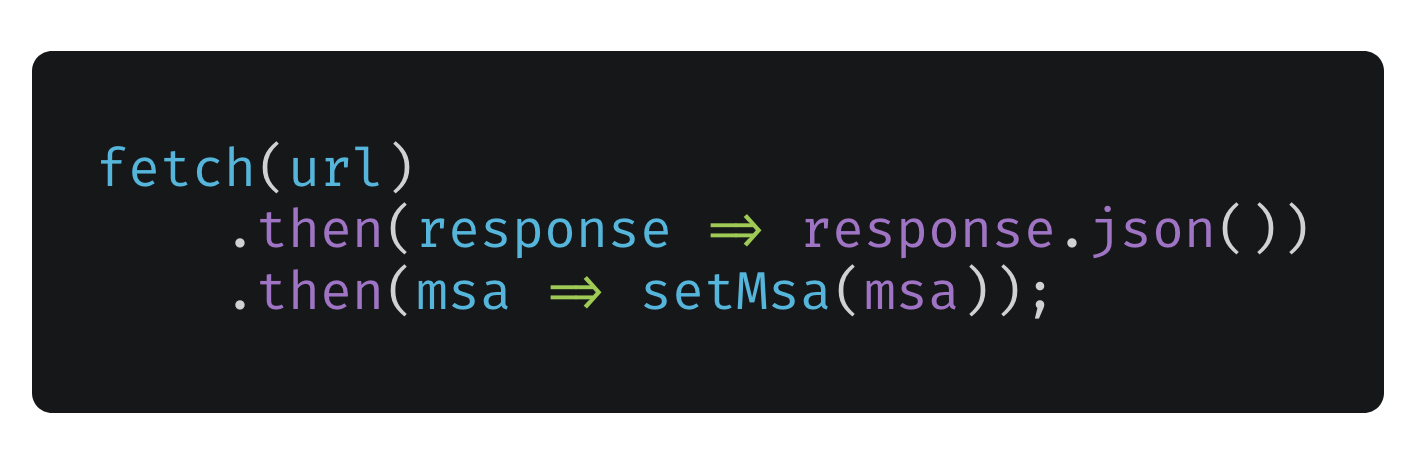
\includegraphics[
            width=.5\linewidth,
        ]{figures/fetch.png}
    \end{figure}
\end{frame}

\begin{frame}{Assignment 2 {\small continued}}
    Add an existing MSA component from \texttt{react-bio-viz}

    \url{https://github.com/genenotebook/react-bio-viz}

    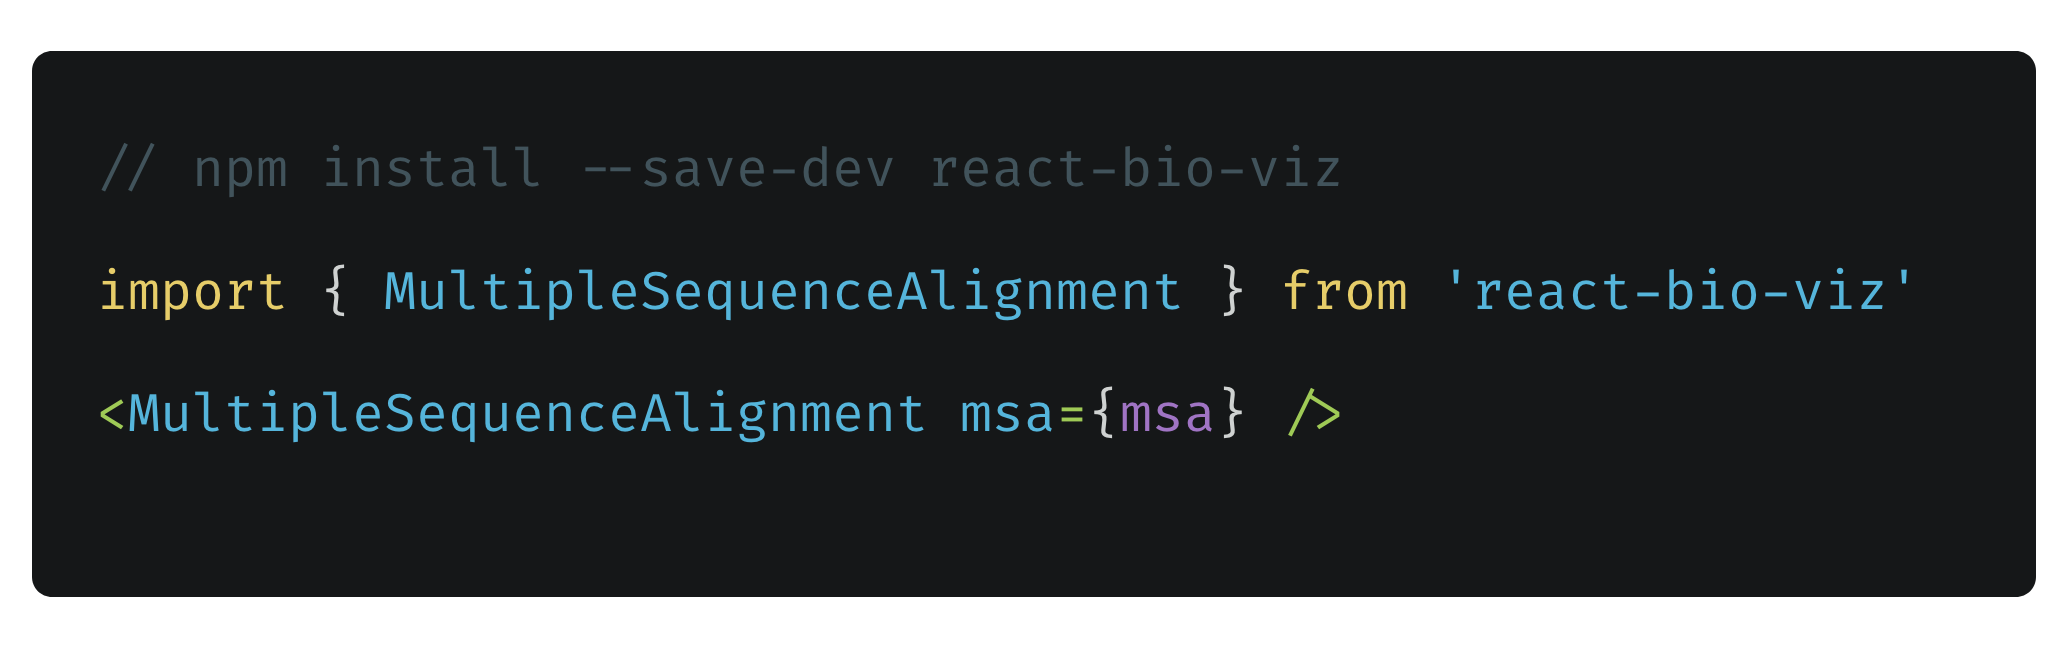
\includegraphics[
        width=.8\linewidth,
    ]{figures/rbv-msa.png}
\end{frame}

\begin{frame}{Assignment 2 {\small continued}}
    Responding to changing dependencies

    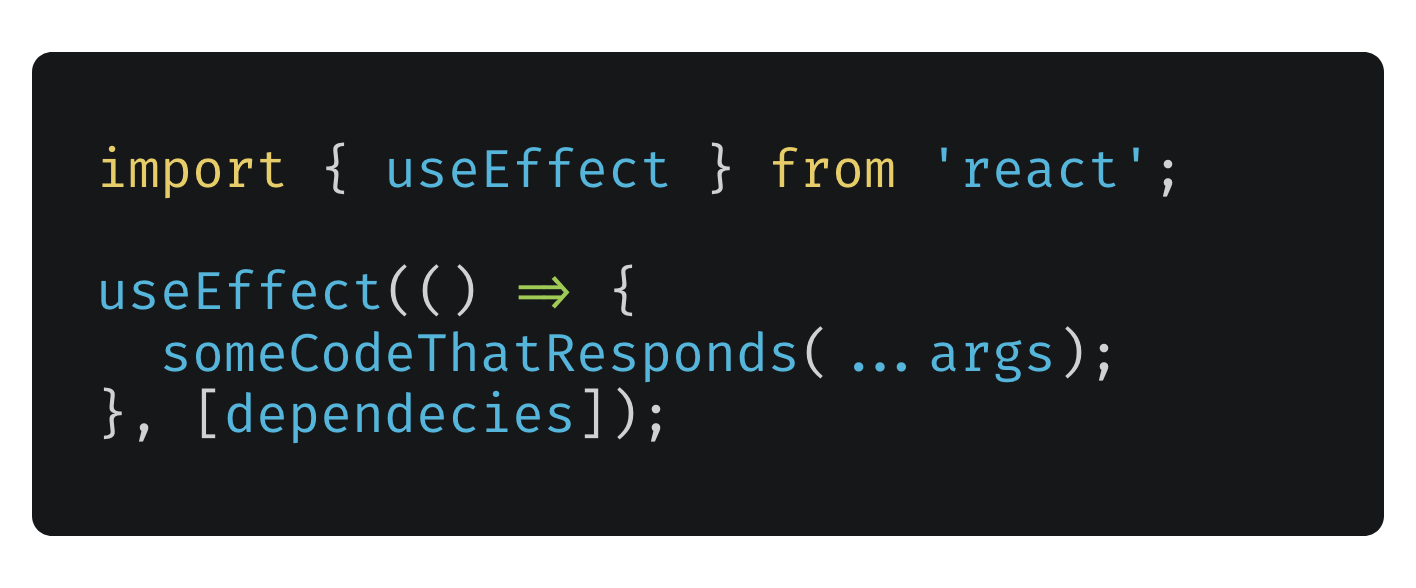
\includegraphics[
        width=.8\linewidth,
    ]{figures/use-effect.png}
\end{frame}

\begin{frame}{Conclusions}
    \begin{itemize}
        \item Modern JS focuses on re-usable components
        \item Toolchains help developers, obscure technical details
    \end{itemize}
\end{frame}

\end{document}

